\documentclass[conference]{IEEEtran}
\IEEEoverridecommandlockouts
% The preceding line is only needed to identify funding in the first footnote. If that is unneeded, please comment it out.
\usepackage{cite}
\usepackage{amsmath,amssymb,amsfonts}
\usepackage{algorithmic}
\usepackage{graphicx}
\usepackage{textcomp}
\usepackage{xcolor}
\def\BibTeX{{\rm B\kern-.05em{\sc i\kern-.025em b}\kern-.08em
    T\kern-.1667em\lower.7ex\hbox{E}\kern-.125emX}}
\begin{document}

\title{Comparison of Machine Learning Techniques to Predict Student Grades Based on Lifestyle\\
}

\author{\IEEEauthorblockN{Samridhi Chaubey}
\IEEEauthorblockA{\textit{Department of Information Technology} \\
\textit{Indira Gandhi Delhi Technical University for Women}\\
Delhi, India\\
samridhi.chaubey@gmail.com}
\and
\IEEEauthorblockN{Priyam Bansal}
\IEEEauthorblockA{\textit{Department of Information Technology} \\
\textit{Indira Gandhi Delhi Technical University for Women}\\
Delhi, India \\
priyambansal66@gmail.com}
}

\maketitle

\begin{abstract}
The present work intends to approach student's academic achievement using Data Mining techniques. Although the results show that a good predictive accuracy can be achieved, if the first and/or second school period grades are available, analysis has shown that there are also other relevant features. As an outcome of this research, more efficient student prediction tools can be developed to improve the quality of education and enhance school resource management.
\end{abstract}

\begin{IEEEkeywords}
Education, Classification and Regression, Decision Trees, Random Forests
\end{IEEEkeywords}

\section{Introduction}
Education is an integral part in shaping an individual's lifestyle and social status. A student's academic performance in formative years is as important as that in later stage after choosing the major. As much as the intelligence and intellect are to play a part, there are many factors associated with the lifestyle of the student that reflect on the academic performance. The aim of this study is to explore how the academic performance of a student is affected by his/her private life by examining in detail, personal information of students with a mean age of ~17 years and find out what influences their grades the most. Three predictive models were used to find the grade of a student, given his personal information and compare their results.

\section{Literature Survey}
This study uses the information collected during 2005-2006 school year from two schools in Portugal Gabriel Pereira and Mousinho da Silveira used by Cortex et. al\cite{cortez2008using} and available on Kaggle\cite{Doe:2009:Online}. The final data consists of two datasets related to Mathematics (with 395 examples) and the Portuguese language (649 records) classes. Cortex et. al used four DM models (i.e. Decision Trees, Random Forest, Neural Networks
and Support Vector Machines) and three input selections (e.g. with and without previous grades) were tested using R. This study uses another model Elastic Net Regularization as a base for Random Forest and Support Vector Machine models and is implemented in python. Elastic net\cite{zou2005regularization} is a regularization method where it is seen to be more efficient and effective than lasso. The elastic net works more efficiently in the cases where the number of predictors is much bigger than the number of observations or when there are a bunch of variables which are independent in nature, but correlated by values in the dataset.

\section{Methodology}
\subsection{Student Data}
Cortez et. all\cite{cortez2008using} collected data from two schools in Portugal from two sources: school reports and questionnaire from a total of 649 students between the ages 15 to 22. The final data consists of two datasets related to Mathematics (with 395 examples) and the Portuguese language (649 records) classes. Table 1 shows the details of all the attributes present in the dataset.

\subsection{Data Pre-processing}
The aim of this study is to predict the final grade G3. The distribution of G3 throughout the dataset is shown in figure 1.
Since the main dataset comprised of two different datasets, each pertaining to the two different courses- Maths and Portuguese, the two datasets were first combined and the duplicates were removed to get a combined dataset. The qualitative variables were changed into numeric values and the target variable- G3 was separated from the other features. \\
For each model, G3 was predicted in the following ways:
\begin{itemize}
    \item Removing G1 and G2
    \item Keeping G1 and removing G2
    \item Keeping G2 and removing G1
    \item Keeping G1 and G2
\end{itemize}
\begin{table}[htbp]
\caption{Student Related Variables}
\begin{center}
\begin{tabular}{|p{1cm}|p{7cm}|}
\hline
\textbf{Attribute} & \textbf{Description} \\
\hline
school&student's school (binary: 'GP'  or 'MS')\\
\hline
sex&student's sex (binary: 'F' - female or 'M' - male)\\
\hline
age&student's age (numeric: from 15 to 22)\\
\hline
address&student's home address type (binary: 'U' - urban or 'R' - rural)\\
\hline
famsize&family size (binary: 'LE3' - less or equal to 3 or 'GT3' - greater than 3)\\
\hline
Pstatus&parent's cohabitation status (binary: 'T' - living together or 'A' - apart)\\
\hline
Medu&mother education (numeric: 0 - 4)\\
\hline
Fedu&father education (numeric: 0 - 4)\\
\hline
Mjob&mother job (nominal)\\
\hline
Fjob&father job (nominal)\\
\hline
reason&reason to choose this school (nominal)\\
\hline
guardian&student's guardian (nominal: 'mother', 'father' or 'other')\\
\hline
traveltime&home to school travel time (numeric: 1 - 4)\\
\hline
studytime&weekly study time (numeric: 1 - 4)\\
\hline
failures&number of past class failures (numeric)\\
\hline
schoolsup&extra educational support (binary: yes or no)\\
\hline
famsup&family educational support (binary: yes or no)\\
\hline
paid&extra paid classes(binary: yes or no)\\
\hline
activities&extra-curricular activities (binary: yes or no)\\
\hline
nursery&attended nursery school (binary: yes or no)\\
\hline
higher&wants to take higher education (binary: yes or no)\\
\hline
internet&Internet access at home (binary: yes or no)\\
\hline
romantic&with a romantic relationship (binary: yes or no)\\
\hline
famrel&quality of family relationships (numeric: from 1 - 5)\\
\hline
freetime&free time after school (numeric: from 1 - 5)\\
\hline
goout&going out with friends (numeric: from 1 - 5)\\
\hline
Dalc&workday alcohol consumption (numeric: from 1 - 5)\\
\hline
Walc&weekend alcohol consumption (numeric: from 1 - 5)\\
\hline
health&current health status (numeric: from 1 - 5)\\
\hline
absences&number of school absences (numeric: from 0 to 93)\\
\hline
G1&first period grade (numeric: from 0 to 20)\\
\hline
G2&second period grade (numeric: from 0 to 20)\\
\hline
G3 &final grade (numeric: from 0 to 20)\\
\hline
\end{tabular}
\end{center}
\label{tab1}
\end{table}

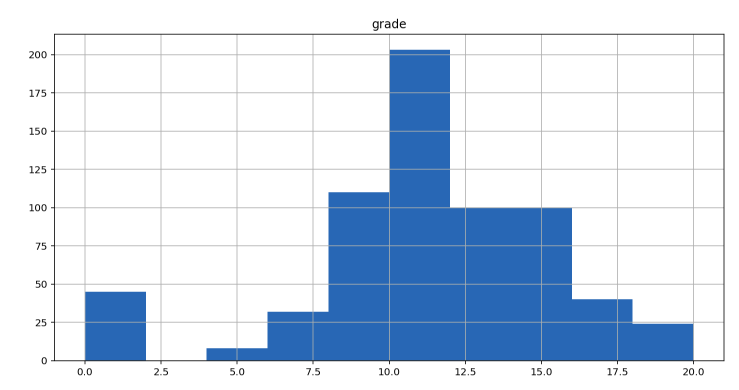
\includegraphics[height=6cm,width=8.8cm]{graph.png}
\begin{center}Figure 1: Distribution of G3\end{center}
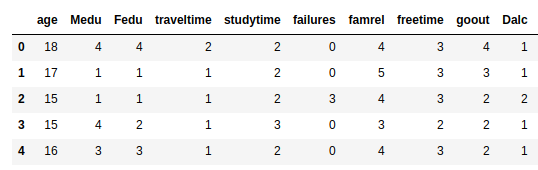
\includegraphics[height=4cm,width=9cm]{table.png}
\begin{center}Figure 2: Conversion of Qualitative Variables into Numerical\end{center}
\subsection{Predictive Models}
After removing G1 and G2, elastic net regularization method was used to get the initial base model on which the improvement of the other models can be seen. To reduce the number of features, correlation between all the features was calculated and any if any two features were found to have correlation value \textgreater 0.9, one of the features was deleted.
It was seen that this did not result in any improvement in the result. To get an improved result, the contribution of every feature to the target variable was calculated and created a model with features that gave us the best contribution.\\
This new data was used by keeping - G1 but not G2, G2 but not G1 and both G1 and G2 on various regression models.\\
Several Data Mining algorithms, each one with its own purpose and capabilities, have been proposed for classification and regression tasks. The Decision Tree is a branching structure that represents a set of rules, distinguishing values in a hierarchical form. This representation can translated into a set of IF-THEN rules, which are easy to understand by humans. The Random Forest (RF) \cite{breiman2001random}(Breiman 2001) is an ensemble of T unpruned DT. Each tree is based in a random feature selection from bootstrap training samples and the RF predictions are built by averaging the outputs of the T trees. The RF is more difficult to interpret when compared with the single DT, although it is still possible to provide explanatory knowledge in terms of its input variable relevance. Support Vector Machines (SVM) has also been proposed for DM tasks\cite{trevor2009elements} (Hastie et al. 2001), obtaining better results when a high non-linearity is present. SVM uses model representations that are difficult to understand by humans.\\
\subsubsection{Elastic Net Regularization}

Elastic net is a hybrid of ridge regression and lasso regularization. This technique can outperform lasso on data with highly correlated predictors. Since the data had a less number of features, which were not highly correlated, this approach was used to get a base model with low performance so that the improvement in the further used models could be gauged easily.\\

The parameters used in Elastic Net Regularization are:
\begin{itemize}
    \item alpha: It is the constant that is used to multiply the penalty terms. Its default value is 1.
    \item l1\textunderscore ratio: It is the Elastic Net mixing parameter, with 0 its value ranging between 0 and 1.
\end{itemize}
To tune these hyper parameter values grid search was used. The grid search provided by GridSearchCV exhaustively generates candidates from a grid of parameter values specified with the param\textunderscore grid parameter. It applies cross-validation to select from these parameter values, given by the cv parameter, here set to 5. \\

\subsubsection{Support Vector Regression}

The method of Support Vector Classification when extended to solve regression problem is called Support Vector Regression. It uses a the kernel trick to transform the data and then finds an optimal hyper-plane to predict the outputs. 

The parameters used in Support Vector Regression are:
\begin{itemize}
    \item kernel: It is the type of kernel used
    \item gamma: It is the kernel coefficient
    \item c: It is the penalty parameter C of the error term.
    \item epsilon: It is the margin of tolerance.
\end{itemize}

Again, to tune gamma and c values grid search was used with cv parameter set to 5. The kernel used was RBF (Radial Basis Function) and epsilon value was set as 0.002. \\

\subsubsection{Random Forest Regression}

Random forest is a meta estimator which works by fitting numerous decision trees on various sub-samples of the dataset. To improve the predictive accuracy and avoid over-fitting averaging is used.

The parameters used in Random Forest Regression are:
\begin{itemize}
    \item max\textunderscore depth: It is the maximum depth of the tree.
    \item n\textunderscore estimators: It is the number of trees in the forest.
\end{itemize}
Again, to tune these hyper parameters grid search was used with cv parameter set to 5.

\section{Result}
The performance of the models was analyzed by calculating R square coefficient of determination for each case. R square can be interpreted to be a statistical measure to determine how closely the data points fit the regression line proposed by the model.
The coefficient value of 0 indicates that that the model is not able to explain the variability of the response data around its mean.
While the coefficient value of 1 indicates that the model is able to explain all the variability of the response data around its mean.\\
The tables show the result.
\begin{table}[!htbp]
\caption{Features Selection}
\begin{tabular}{|p{5cm}|p{3cm}|}
\hline
\textbf{ } & \textbf{Average R square} \\
\hline
Normal Elastic Net Regularization&0.0515\\
\hline
Removing highly correlated features&0.0515\\
\hline
Best contribution features&0.0584\\
\hline
\end{tabular}
\label{tab1}
\end{table}
The table clearly indicates that by removing the features that are highly correlated to one another is irrelevant because the average R square value did not improve but stayed the same.
But when the contribution of each feature to the target variable was considered, improvement in performance was observed.
\\The table shows another set of result
\begin{table}[!htbp]
\caption{Average of our R square value}
\begin{tabular}{|p{4.25cm}|p{1cm}|p{1cm}|p{1cm}|}
\hline
\textbf{ } & \textbf{ENR} & \textbf{SVR} & \textbf{RF} \\
\hline
Without G1 and G2&0.0584&-0.0375&0.0341\\
\hline
With G1 and without G2&0.828&0.516&0.576\\
\hline
Without G1 and with G2&0.827&0.806&0.814\\
\hline
With both G1 and G2&0.829&0.800&0.800\\
\hline
\end{tabular}
\label{tab1}
\end{table}
\\Improvement in the value of average R square coefficient was seen when moving from Elastic Net Regularization model to Support Vector Regression model and further to Random Forest Regression model.
\\It can also be seen that prediction is more accurate when features like G1 or G2 were included than when both of them were eliminated.
\section*{Discussion}
The results do not show a very strong relationship between a student's lifestyle and grades initially. With the use of advanced Data Mining algorithms, however, there is a visible improvement. Moreover, daily habits and lifestyle do have a great impact on academics in practical life. It can be argued that with a more diverse data set i.e data from different countries, covering more number of schools and thus comprising of a greater number of students, better results can be generated.


\bibliographystyle{IEEEtran}
\bibliography{refer} 

\iffalse
\newpage
\begin{flushleft}
\textbf{{\Large REFERENCES}}
\end{flushleft}

\begin{itemize}
  \cite{}
\end{itemize}

\fi
\end{document}